\documentclass[12pt,a4paper]{article}
\usepackage[utf8]{inputenc}
\usepackage[T1]{fontenc}
\usepackage[serbian]{babel}
\usepackage{amsmath, amssymb}
\usepackage{graphicx}
\usepackage{booktabs}
\usepackage{array}
\usepackage{geometry}
\usepackage{hyperref}
\usepackage{float}
\usepackage{caption}
\usepackage{listings}
\usepackage{xcolor}

\geometry{a4paper, top=2.5cm, bottom=2.5cm, left=2.8cm, right=2.5cm}

\hypersetup{colorlinks=true, linkcolor=blue, urlcolor=blue, citecolor=blue}

\lstdefinestyle{matlab}{
	language=Matlab,
	basicstyle=\small\ttfamily,
	keywordstyle=\color{blue}\bfseries,
	commentstyle=\itshape\color{green!50!black},
	stringstyle=\color{orange!80!black},
	numbers=left,
	numberstyle=\tiny\color{gray},
	frame=tb,
	breaklines=true,
	tabsize=2,
	showstringspaces=false
}

\begin{document}
	
	%=================================================================
	% NASLOVNA STRANA
	%=================================================================
	\begin{titlepage}
		\centering
		\vspace*{1.5cm}
		{\large Matematički fakultet, Univerzitet u Beogradu}\\[0.3cm]
		{\large Predmet: Osnove matematičkog modeliranja}\\[2cm]
		{\Huge\bfseries Grip}\\[0.5cm]
		{\Large SIR model}\\[2cm]
		{\large Seminarski rad}\\[3.5cm]
		\begin{flushright}
			{\large Autori: Nikola Stanojević 107/2022}\\[0.8cm]
			{\large Mlađan Simić 90/2022}\\[0.8cm]
		\end{flushright}
		\vfill
		{\large Beograd, \the\year.}
	\end{titlepage}
	
	%=================================================================
	\tableofcontents
	\newpage
	%=================================================================
	
	%=================================================================
	\section{Uvod}
	%=================================================================
	
	Grip je zarazna bolest disajnih puteva koju izazivaju virusi influence tipa A, B i C.
	Svake godine, tokom zimske sezone, grip zahvata između 10\% i 20\% svetske populacije i odgovoran
	je za 290\,000 do 650\,000 smrtnih ishoda godišnje \cite{WHO2019}. Razumevanje dinamike širenja
	zaraznih bolesti od ključnog je značaja za planiranje javnozdravstvenih mera i procenu efikasnosti
	različitih intervencija.
	
	Matematičko modeliranje epidemija ima dugu istoriju. Kermack i McKendrick su 1927. godine uveli
	prvi deterministički kompartmentalni model koji deli populaciju na odelite grupe prema zdravstvenom
	statusu \cite{Kermack1927}. Ovaj pristup danas poznat kao SIR model (od eng.\ 
	\textit{Susceptible}--\textit{Infected}--\textit{Recovered}) i dalje je osnova savremene 
	matematičke epidemiologije.
	
	U ovom radu formulišemo i analiziramo SIR model za sezonski grip u zatvorenoj populaciji.
	\begin{itemize}
		\item U Odeljku~\ref{sec:model} izvodimo sistem diferencijalnih jednačina koji opisuje
		dinamiku bolesti i definišemo sve veličine i parametre modela.
		\item U Odeljku~\ref{sec:params} procenjujemo vrednosti parametara modela na osnovu
		empirijskih podataka o epidemiji u gradu sa $N=15\,000$ stanovnika.
		\item Odeljak~\ref{sec:ravnoteza} posvećen je analizi ravnotežnih tačaka i određivanju
		uslova pod kojima broj zaraženih počinje da opada, uz poređenje sa podacima.
		\item U Odeljku~\ref{sec:scenariji} razmatramo tri scenarija kontrole širenja virusa
		-- vakcinaciju, karantin i primenu lekova -- i poredimo ih sa osnovnim slučajem.
		\item Odeljak~\ref{sec:zakljucak} sadrži zaključna razmatranja i preporuke.
	\end{itemize}
	Grafički rezultati su dobijeni numeričkim rešavanjem sistema diferencijalnih jednačina u
	MATLAB-u.
	
	%=================================================================
	\section{Matematički model}
	\label{sec:model}
	%=================================================================
	
	\subsection{Pretpostavke modela}
	
	Posmatramo \textbf{zatvorenu} populaciju ukupnog broja $N$ jedinki u toku jedne sezone gripa.
	Pretpostavljamo da infekcija jednim sojem virusa daje trajni imunitet na taj soj, pa ne dolazi
	do ponovne zaraze. Pored toga, zanemarujemo rađanje, prirodne smrtne slučajeve i migracije,
	budući da je posmatrani vremenski period kratak (30 dana).
	
	Svakom pojedincu u svakom trenutku $t$ pripisujemo jedno od tri stanja:
	\begin{itemize}
		\item \textbf{Zdravi -- $S$} (engl.\ \textit{Susceptible}): podložni zarazi, još nisu bili
		izloženi virusu ili nemaju imunitet.
		\item \textbf{Zaraženi -- $I$} (engl.\ \textit{Infected}): trenutno bolesni i sposobni da
		prenesu bolest na zdrave.
		\item \textbf{Oporavljeni -- $R$} (engl.\ \textit{Recovered}): preležali bolest i stekli
		imunitet; ne mogu biti ponovo zaraženi istim sojem.
	\end{itemize}
	
	Neka $S(t)$, $I(t)$ i $R(t)$ označavaju \textit{udeo} (frakciju) zdravih, zaraženih i
	oporavljenih u ukupnoj populaciji $N$ u trenutku $t$. Odgovarajući apsolutni brojevi su
	$N\cdot S(t)$, $N\cdot I(t)$ i $N\cdot R(t)$. Pošto svaki pojedinac u svakom trenutku pripada
	tačno jednoj grupi, važi uslov konzervacije:
	\begin{equation}
		S(t) + I(t) + R(t) = 1, \quad \forall\, t \geq 0.
		\label{eq:konz}
	\end{equation}
	
	Pretpostavlja se da je populacija \textbf{homogeno izmešana}: verovatnoća da se bilo koja dva
	pojedinca sretnu je jednaka za sve parove, pa je stopa novih zaraza proporcionalna produktu
	broja zdravih i zaraženih osoba.
	
	\subsection{Sistem diferencijalnih jednačina}
	
	Brzina prenošenja bolesti proporcionalna je broju kontakata između zdravih i zaraženih, tj.\
	produktu $S(t)\cdot I(t)$, sa koeficijentom proporcionalnosti $a > 0$:
	\begin{equation}
		\frac{\mathrm{d}S}{\mathrm{d}t} = -a\,S(t)\,I(t).
		\label{eq:dS}
	\end{equation}
	Brzina oporavka proporcionalna je broju zaraženih sa koeficijentom $r > 0$, dok istovremeno
	zaraženi nastaju prelaskom iz grupe zdravih. Stoga:
	\begin{equation}
		\frac{\mathrm{d}I}{\mathrm{d}t} = a\,S(t)\,I(t) - r\,I(t).
		\label{eq:dI}
	\end{equation}
	Promena udela oporavljenih jednaka je stopi oporavka:
	\begin{equation}
		\frac{\mathrm{d}R}{\mathrm{d}t} = r\,I(t).
		\label{eq:dR}
	\end{equation}
	
	Sabiranjem \eqref{eq:dS}--\eqref{eq:dR} dobija se
	$\frac{\mathrm{d}}{\mathrm{d}t}(S+I+R)=0$,
	što potvrđuje konzervacioni uslov \eqref{eq:konz}. Sistem je kompletno određen početnim
	uslovima:
	\begin{equation}
		S(0) = S_0,\quad I(0) = I_0,\quad R(0) = R_0,
		\quad S_0+I_0+R_0 = 1.
		\label{eq:IC}
	\end{equation}
	
	Parametri modela imaju jasnu epidemiološku interpretaciju:
	\begin{itemize}
		\item $a\;[\mathrm{dan}^{-1}]$ -- stopa prenošenja: objedinjuje učestalost kontakata i
		verovatnoću prenosa infekcije pri jednom kontaktu.
		\item $r\;[\mathrm{dan}^{-1}]$ -- stopa oporavka: recipročna vrednost $1/r$ je prosečno
		vreme trajanja bolesti u danima.
	\end{itemize}
	
	\subsection{Osnovni reprodukcioni broj}
	
	\textbf{Osnovni reprodukcioni broj} $\mathcal{R}_0$ definišemo kao prosečan broj sekundarnih
	zaraza koje prouzrokuje jedan zaraženi pojedinac u potpuno zdravoj populaciji. Za SIR model:
	\begin{equation}
		\mathcal{R}_0 = \frac{a\,S_0}{r}.
		\label{eq:R0def}
	\end{equation}
	Ako je $\mathcal{R}_0 > 1$, infekcija se širi (epidemija); ako je $\mathcal{R}_0 \leq 1$, bolest
	se gasi bez epidemije.
	
	Napominjemo da je ovaj SIR model autonomni sistem nelinearnih običnih diferencijalnih jednačina prvog reda čije egzaktno
	rešenje u zatvorenom obliku ne postoji, pa se rešava numerički (videti Prilog).
	
	%=================================================================
	\section{Procena parametara modela}
	\label{sec:params}
	%=================================================================
	
	\subsection{Podaci}
	
	U gradu sa $N=15\,000$ stanovnika vođena je evidencija broja zaraženih $\tilde{I}(t)$ i broja
	oporavljenih $\tilde{R}(t)$ tokom 30 dana. Podaci su prikazani u Tabeli~\ref{tab:podaci},
	a odgovarajući udeli su $I(t)=\tilde{I}(t)/N$, $R(t)=\tilde{R}(t)/N$ i $S(t)=1-I(t)-R(t)$.
	
	\begin{table}[H]
		\centering
		\caption{Broj zaraženih $\tilde{I}(t)$ i oporavljenih $\tilde{R}(t)$ osoba u gradu sa $N=15\,000$ stanovnika tokom perioda od 30 dana.}
		\label{tab:podaci}
		\small
		\setlength{\tabcolsep}{5pt}
		\begin{tabular}{crrcrrcrrcrr}
			\toprule
			$t$ & $\tilde{I}$ & $\tilde{R}$ && $t$ & $\tilde{I}$ & $\tilde{R}$ && $t$ & $\tilde{I}$ & $\tilde{R}$ \\
			\midrule
			0  & 150  & 0     && 10 & 2150 & 2528  && 20 & 1288 & 10615 \\
			1  & 205  & 51    && 11 & 2474 & 3255  && 21 & 1043 & 11051 \\
			2  & 280  & 120   && 12 & 2726 & 4091  && 22 & 832  & 11403 \\
			3  & 378  & 214   && 13 & 2861 & 5012  && 23 & 663  & 11685 \\
			4  & 508  & 341   && 14 & 2855 & 5978  && 24 & 519  & 11908 \\
			5  & 674  & 512   && 15 & 2724 & 6943  && 25 & 406  & 12084 \\
			6  & 887  & 740   && 16 & 2492 & 7864  && 26 & 318  & 12222 \\
			7  & 1150 & 1040  && 17 & 2197 & 8706  && 27 & 246  & 12330 \\
			8  & 1454 & 1428  && 18 & 1882 & 9449  && 28 & 193  & 12414 \\
			9  & 1797 & 1920  && 19 & 1573 & 10084 && 29 & 148  & 12479 \\
			\bottomrule
		\end{tabular}
	\end{table}
	
	\subsection{Metoda procene parametara}
	
	Parametre $r$ i $a$ procenjujemo aproksimacijom izvoda metodom \textbf{konačnih razlika unapred}, $\frac{\mathrm{d}f}{\mathrm{d}t}\big|_{t} \approx f(t+1)-f(t)$,
	primenjenom na diskretne podatke sa korakom $\Delta t = 1\;\mathrm{dan}$.
	
	\paragraph{Procena koeficijenta oporavka $r$.}
	Iz jednačine~\eqref{eq:dR}:
	\begin{equation}
		r \approx \frac{R(t+1)-R(t)}{I(t)} = \frac{\tilde{R}(t+1)-\tilde{R}(t)}{\tilde{I}(t)},
		\quad t = 0,1,\ldots,28.
		\label{eq:r_est}
	\end{equation}
	U drugoj jednakosti se $N$ krati. Nekoliko primera:
	\[
	t=0:\;\frac{51}{150}=0{,}340;\quad
	t=1:\;\frac{69}{205}=0{,}337;\quad
	t=2:\;\frac{94}{280}=0{,}336;\quad
	t=3:\;\frac{127}{378}=0{,}336.
	\]
	Vrednosti su izuzetno konzistentne duž celog niza. Računanjem srednje vrednosti svih 29 procena po 
	formuli~\eqref{eq:r_est} dobija se:
	\begin{equation}
		\boxed{r \approx 0{,}336\;\mathrm{dan}^{-1},}
		\label{eq:r_val}
	\end{equation}
	što odgovara prosečnom trajanju bolesti od $1/r \approx 2{,}98 \approx 3$ dana.
	
	\paragraph{Procena koeficijenta prenošenja $a$.}
	Iz jednačine~\eqref{eq:dI}, izražavanjem $a$:
	\begin{equation}
		a \approx \frac{[I(t+1)-I(t)] + r\,I(t)}{S(t)\,I(t)}
		= \frac{[\tilde{I}(t+1)-\tilde{I}(t)] + r\,\tilde{I}(t)}{\tilde{S}(t)\,\tilde{I}(t)/N},
		\label{eq:a_est}
	\end{equation}
	gde je $\tilde{S}(t)=N-\tilde{I}(t)-\tilde{R}(t)$. Primeri:
	
	\begin{center}
		\setlength{\tabcolsep}{8pt}
		\begin{tabular}{cccc}
			\toprule
			$t$ & $\tilde{S}(t)$ & Brojilac & $a_t$ \\
			\midrule
			0 & 14850 & $55+50{,}4=105{,}4$ & $0{,}710$ \\
			1 & 14744 & $75+68{,}9=143{,}9$ & $0{,}714$ \\
			2 & 14600 & $98+94{,}1=192{,}1$ & $0{,}705$ \\
			3 & 14408 & $130+127{,}0=257{,}0$ & $0{,}707$ \\
			4 & 14151 & $166+170{,}7=336{,}7$ & $0{,}710$ \\
			5 & 13814 & $213+226{,}5=439{,}5$ & $0{,}710$ \\
			\bottomrule
		\end{tabular}
	\end{center}
	
	Procena je stabilna tokom faze rasta epidemije (dani 0--12). Srednja vrednost:
	\begin{equation}
		\boxed{a \approx 0{,}71\;\mathrm{dan}^{-1}.}
		\label{eq:a_val}
	\end{equation}
	
	\subsection{Početni uslovi i osnovni reprodukcioni broj}
	
	Na osnovu podataka za $t=0$:
	\begin{equation}
		I_0 = \frac{150}{15000} = 0{,}010,\quad
		R_0 = 0,\quad
		S_0 = 1-I_0-R_0 = 0{,}990.
	\end{equation}
	
	Osnovni reprodukcioni broj za ove parametre:
	\begin{equation}
		\mathcal{R}_0 = \frac{a\,S_0}{r} = \frac{0{,}71\times 0{,}99}{0{,}336} \approx 2{,}09.
		\label{eq:R0_val}
	\end{equation}
	Vrednost $\mathcal{R}_0\approx 2{,}09 > 1$ potvrđuje epidemijski karakter pojave: svaki zaraženi
	u proseku zarazi još dvoje zdravih. Grafički prikaz rešenja modela sa procenjenim parametrima,
	poređen sa podacima iz Tabele~\ref{tab:podaci}, dat je na Slici~\ref{fig:sir_basic}.
	
	\begin{figure}[H]
		\centering
		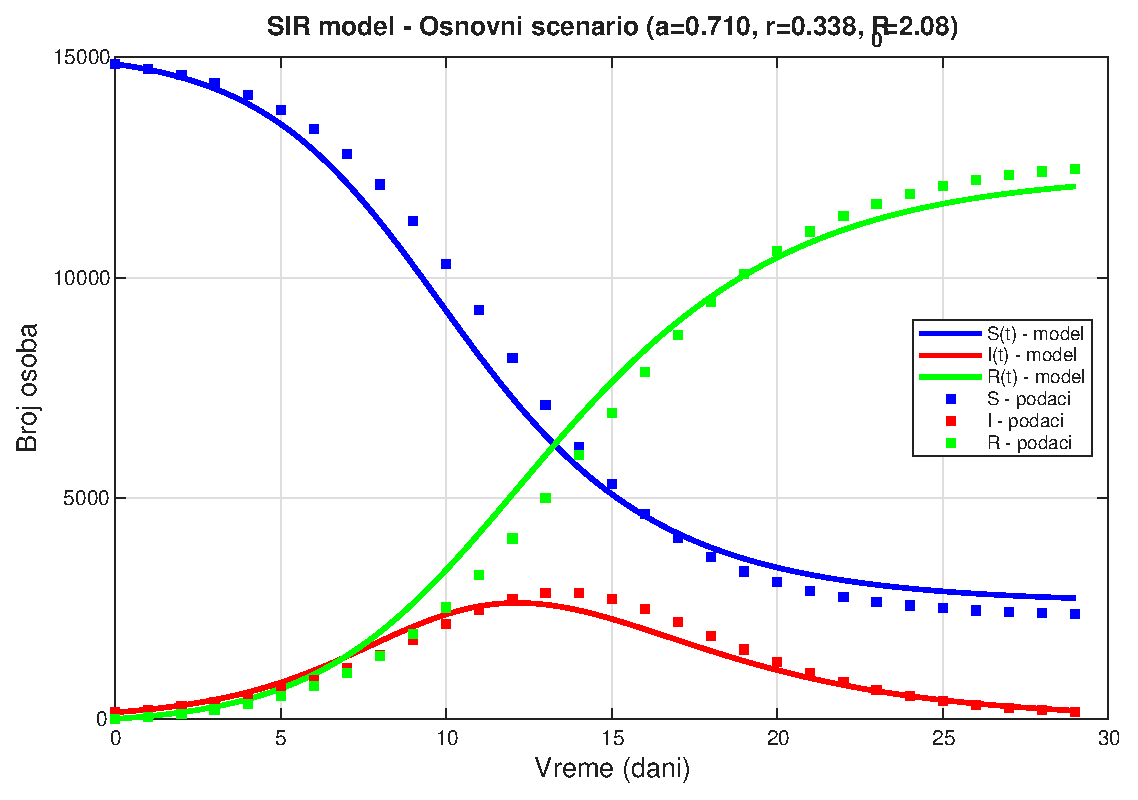
\includegraphics[width=0.82\textwidth]{fig_basic.eps}
		\caption{Rešenje SIR modela sa procenjenim parametrima ($a=0{,}71$, $r=0{,}336$) poređeno
			sa podacima. Pune linije -- numeričko rešenje; markeri ($\square$) -- podaci.}
		\label{fig:sir_basic}
	\end{figure}
	
	%=================================================================
	\section{Ravnotežne tačke i uslovi za smanjenje zaraze}
	\label{sec:ravnoteza}
	%=================================================================
	
	\subsection{Ravnotežne tačke}
	
	Ravnotežne (stacionarne) tačke sistema \eqref{eq:dS}--\eqref{eq:dR} su tačke $(S^*, I^*, R^*)$
	u kojima su sve tri desne strane jednake nuli:
	\begin{alignat}{2}
		&-a\,S^* I^* = 0, \label{eq:eq1}\\
		&\;a\,S^* I^* - r\, I^* = 0, \label{eq:eq2}\\
		&\;r\,I^* = 0. \label{eq:eq3}
	\end{alignat}
	Iz \eqref{eq:eq3}, pošto je $r>0$, sledi $I^*=0$. Supstitucijom $I^*=0$ u \eqref{eq:eq1}
	i \eqref{eq:eq2} one su identički zadovoljene za bilo koje $S^*$. Jedini ograničavajući
	uslov je neganatnost i normalizacija: $S^*, R^* \geq 0$ i $S^*+R^*=1$.
	
	Skup ravnotežnih tačaka čine sva stanja bez zaraženih:
	\begin{equation}
		\mathcal{E} = \bigl\{(S^*,\;0,\;1-S^*)\;:\; S^*\in[0,1]\bigr\}.
	\end{equation}
	Svaka tačka iz $\mathcal{E}$ opisuje situaciju bez zaraženih: udeo $S^*$ populacije ostao je
	zdrav, a udeo $1-S^*$ se oporavio i stekao imunitet. Iz ovoga sledi da se SIR epidemija 
	\textit{uvek završava} -- broj zaraženih neminovno teži nuli, bez obzira na početne uslove.
	Epidemija ne može trajati beskonačno (endemski scenario nije moguć u ovom modelu).
	
	\subsection{Uslov za smanjenje broja zaraženih}
	
	Broj zaraženih $I(t)$ opada kada je $\mathrm{d}I/\mathrm{d}t<0$. Iz \eqref{eq:dI}:
	\begin{equation}
		\frac{\mathrm{d}I}{\mathrm{d}t} = I(t)\,\bigl(a\,S(t)-r\bigr) < 0.
	\end{equation}
	Pošto je $I(t)>0$ dok epidemija traje, uslov se svodi na:
	\begin{equation}
		\boxed{S(t) < \frac{r}{a}.}
		\label{eq:uslov_pad}
	\end{equation}
	Supstituišući procenjene parametre:
	\begin{equation}
		S(t) < \frac{r}{a} = \frac{0{,}336}{0{,}71} \approx 0{,}473.
	\end{equation}
	Broj zaraženih počinje da opada kada manje od \textbf{47,3\%} populacije ostane zdravo, što
	u apsolutnim brojevima iznosi $0{,}473\times 15\,000\approx 7\,095$ osoba.
	
	\subsection{Poređenje sa podacima}
	
	Iz podataka u Tabeli~\ref{tab:podaci} računamo $\tilde{S}(t)=N-\tilde{I}(t)-\tilde{R}(t)$:
	\begin{align*}
		\tilde{S}(13) &= 15000 - 2861 - 5012 = 7127 > 7095,\\
		\tilde{S}(14) &= 15000 - 2855 - 5978 = 6167 < 7095.
	\end{align*}
	Model predviđa da $I(t)$ dostiže maksimum između $t=13$ i $t=14$ dana. Zaista, iz podataka:
	$\tilde{I}(13)=2861$ i $\tilde{I}(14)=2855$ su gotovo jednaki (razlika svega 6 osoba), a od
	$t=15$ nadalje $\tilde{I}(t)$ striktno opada. Pik zaraze desio se na dan $t\approx 13$,
	u odličnoj saglasnosti sa modelom.
	
	\subsection{Konačna veličina epidemije}
	
	Deljenjem \eqref{eq:dS} sa \eqref{eq:dR} eliminišemo vreme:
	\begin{equation}
		\frac{\mathrm{d}S}{\mathrm{d}R} = -\frac{a}{r}\,S
		\quad\Rightarrow\quad
		S(t) = S_0\,\exp\!\left(-\frac{a}{r}\,R(t)\right).
		\label{eq:SR_rel}
	\end{equation}
	(Koristili smo $R(0)=0$.) Kad $t\to\infty$, $I_\infty=0$ pa $R_\infty=1-S_\infty$.
	Supstitucijom u \eqref{eq:SR_rel}:
	\begin{equation}
		S_\infty = S_0\,\exp\!\left(-\frac{a}{r}(1-S_\infty)\right).
		\label{eq:final_size}
	\end{equation}
	Ovo je transcendentna jednačina bez analitičkog rešenja. Numeričkim rešavanjem za naše
	parametre ($S_0=0{,}99$, $a/r=2{,}113$) dobijamo $S_\infty\approx 0{,}164$, tj.\ ukupno
	zaraženih:
	\begin{equation}
		1-S_\infty \approx 83{,}6\% \quad\Rightarrow\quad
		\approx 12\,540 \text{ osoba od } 15\,000.
	\end{equation}
	Iz podataka na $t=29$: $\tilde{S}(29)=15000-148-12479=2373$, tj.\
	$S(29)=0{,}158\approx S_\infty$, što potvrđuje tačnost modela.
	
	%=================================================================
	\section{Scenariji kontrole širenja virusa}
	\label{sec:scenariji}
	%=================================================================
	
	Razmatramo tri mere kontrole, uvek polazeći od istih početnih uslova kao u Odeljku~\ref{sec:params}.
	Prikazujemo modifikovani model, odgovarajući $\mathcal{R}_0$ i numerički simulirani tok bolesti.
	Sve četiri krive (osnovni scenario + tri kontrolna) prikazane su grafički i numerički poređene.
	
	\subsection{Scenario 1: Vakcinacija}
	
	\paragraph{Opis.}
	Pred početak sezone gripa vakciniše se 20\% ukupne populacije (vakcina je 100\% efikasna).
	Vakcinisani odmah dobijaju imunitet i prelaze iz grupe $S$ u grupu $R$.
	
	\paragraph{Modifikovani početni uslovi.}
	Broj vakcinisanih: $0{,}20\times 15000=3000$ osoba, koje prelaze iz $S$ u $R$:
	\begin{equation}
		S_0^{(1)} = 0{,}99 - 0{,}20 = 0{,}79,\quad
		I_0^{(1)} = 0{,}01,\quad
		R_0^{(1)} = 0{,}20.
	\end{equation}
	
	\paragraph{Model.} Jednačine \eqref{eq:dS}--\eqref{eq:dR} nepromenjene; $a=0{,}71$, $r=0{,}336$.
	
	\paragraph{Reprodukcioni broj.}
	\begin{equation}
		\mathcal{R}_0^{(1)} = \frac{a\,S_0^{(1)}}{r}
		= \frac{0{,}71\times 0{,}79}{0{,}336} \approx 1{,}67.
	\end{equation}
	
	Vakcinacijom se $\mathcal{R}_0$ smanjuje sa 2,09 na 1,67. Kako je i dalje $\mathcal{R}_0^{(1)}>1$,
	epidemija nastaje, ali je znatno slabija. Da bi se postigao \textbf{kolektivni imunitet}
	(sprečavanje epidemije), potrebno je vakcinisati udeo
	$p>1-1/\mathcal{R}_0=1-1/2{,}09\approx 52\%$ populacije.
	
	\subsection{Scenario 2: Karantin}
	
	\paragraph{Opis.}
	20\% zaraženih osoba u svakom trenutku nalazi se u karantinu i ne može biti u kontaktu sa
	drugima. Efektivno, samo 80\% zaraženih učestvuje u prenošenju bolesti.
	
	\paragraph{Modifikovani model.}
	Stopa novih zaraza zavisi od kontakata zdravih sa \textit{aktivnim} zaraženima (izvan
	karantina). Efektivni udeo aktivnih zaraženih je $0{,}80\cdot I(t)$, pa:
	\begin{align}
		\frac{\mathrm{d}S}{\mathrm{d}t} &= -a\,S(t)\cdot[0{,}80\cdot I(t)]
		= -a_{\rm ef}^{(2)}\,S(t)\,I(t), \\
		\frac{\mathrm{d}I}{\mathrm{d}t} &= a_{\rm ef}^{(2)}\,S(t)\,I(t) - r\,I(t), \\
		\frac{\mathrm{d}R}{\mathrm{d}t} &= r\,I(t),
	\end{align}
	gde je $a_{\rm ef}^{(2)} = 0{,}80\times 0{,}71 = 0{,}568\;\mathrm{dan}^{-1}$.
	
	\paragraph{Reprodukcioni broj.}
	\begin{equation}
		\mathcal{R}_0^{(2)} = \frac{a_{\rm ef}^{(2)}\cdot S_0}{r}
		= \frac{0{,}568\times 0{,}99}{0{,}336} \approx 1{,}67.
	\end{equation}
	
	\subsection{Scenario 3: Lekovi}
	
	\paragraph{Opis.}
	Svi zaraženi uzimaju adekvatnu terapiju lekovima, čime se verovatnoća ozdravljenja
	povećava za 20\%. Koeficijent oporavka raste:
	\begin{equation}
		r_{\rm ef}^{(3)} = 1{,}20\times r = 1{,}20\times 0{,}336 = 0{,}4032\;\mathrm{dan}^{-1}.
	\end{equation}
	Prosečno trajanje bolesti se skraćuje sa $\approx 3$ na $\approx 2{,}48$ dana.
	
	\paragraph{Model.} Jednačine \eqref{eq:dS}--\eqref{eq:dR} sa $r_{\rm ef}^{(3)}$ umesto $r$;
	parametar $a$ ostaje nepromenjen.
	
	\paragraph{Reprodukcioni broj.}
	\begin{equation}
		\mathcal{R}_0^{(3)} = \frac{a\,S_0}{r_{\rm ef}^{(3)}}
		= \frac{0{,}71\times 0{,}99}{0{,}4032} \approx 1{,}74.
	\end{equation}
	
	\subsection{Grafički prikaz i poređenje scenarija}
	
	Sva četiri scenarija su numerički rešena u MATLAB-u (videti Prilog).
	Slika~\ref{fig:I_svi} prikazuje vremensku evoluciju broja zaraženih $I(t)\cdot N$ za sve
	scenarije, a Tabela~\ref{tab:poredjenje} sadrži ključne veličine.
	
	\begin{figure}[H]
		\centering
		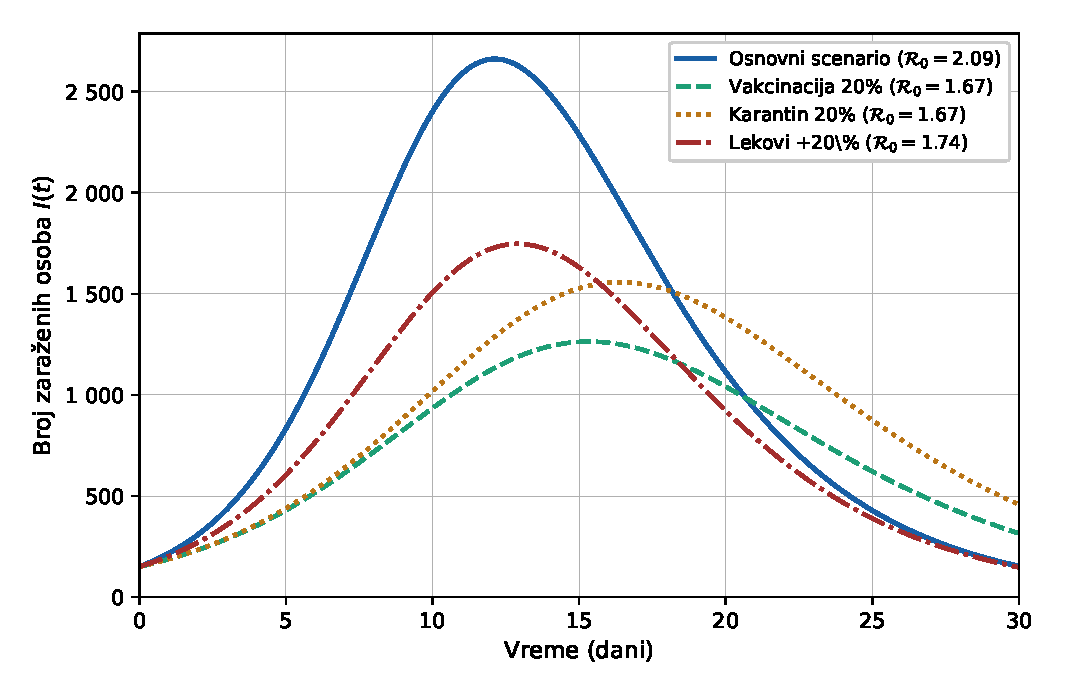
\includegraphics[width=0.88\textwidth]{scenariji/I_t_scenariji.eps}
		\caption{Broj zaraženih $\tilde{I}(t)$ za sva četiri scenarija tokom 30 dana.}
		\label{fig:I_svi}
	\end{figure}

    \begin{figure}[H]
		\centering
		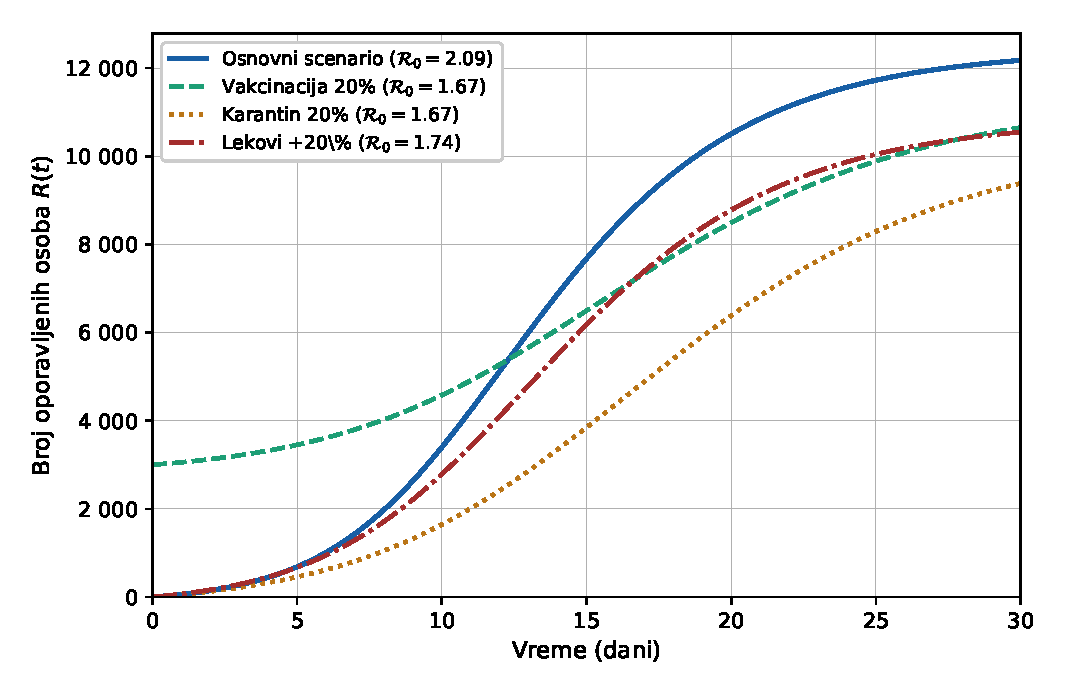
\includegraphics[width=0.88\textwidth]{scenariji/R_t_scenariji.eps}
		\caption{Broj oporavljenih $\tilde{R}(t)$ za sva četiri scenarija tokom 30 dana.}
		\label{fig:R_svi}
	\end{figure}

    \begin{figure}[H]
		\centering
		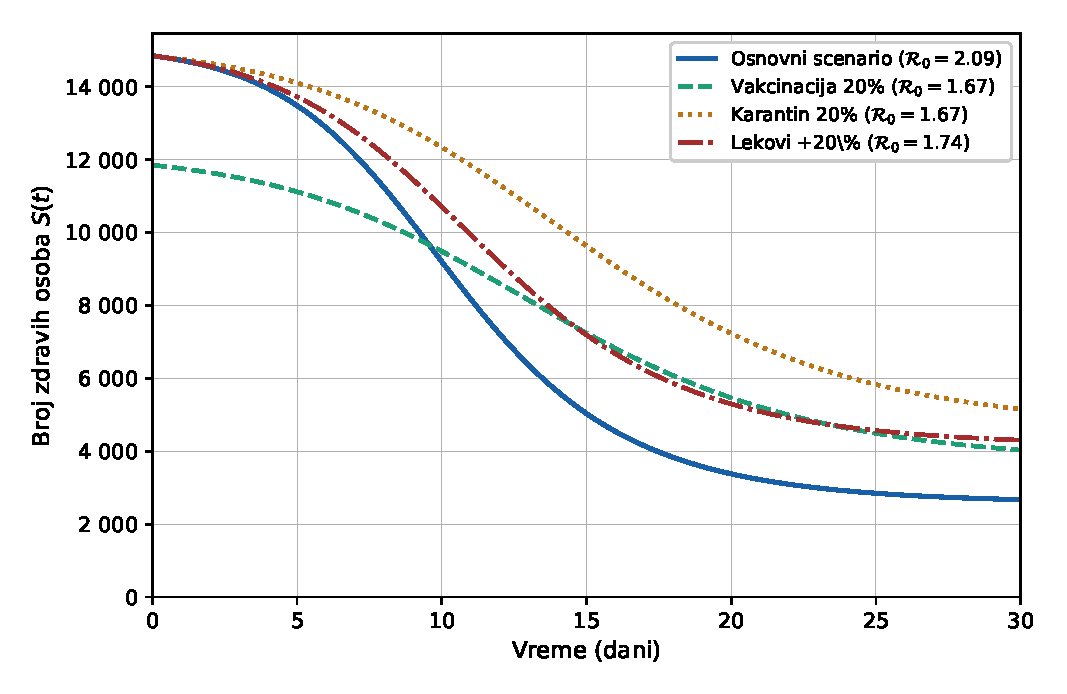
\includegraphics[width=0.88\textwidth]{scenariji/S_t_scenariji.eps}
		\caption{Broj zdravih $\tilde{S}(t)$ za sva četiri scenarija tokom 30 dana.}
		\label{fig:S_svi}
	\end{figure}
	
	\begin{table}[H]
		\centering
		\caption{Poređenje scenarija: osnovni reprodukcioni broj, maksimalni broj zaraženih (i dan dostizanja maksimuma), ukupan broj osoba koje su prebolele grip tokom 30 dana.}
		\label{tab:poredjenje}
		\setlength{\tabcolsep}{9pt}
		\begin{tabular}{lcccc}
			\toprule
			Scenario & $\mathcal{R}_0$ & $\max \tilde{I}(t)$ & Dan maks. & Ukupno zaraženih \\
			\midrule
			0 -- Osnovni    & $2{,}09$ & $\approx 2631$ & $\approx 12$ & $\approx 12262$ \\
			1 -- Vakcinacija & $1{,}67$ & $\approx 1243$ & $\approx 15$ & $\approx 7843$ \\
			2 -- Karantin   & $1{,}67$ & $\approx 1530$ & $\approx 16$ & $\approx 9669$ \\
			3 -- Lekovi      & $1{,}74$ & $\approx 1719$ & $\approx 13$ & $\approx 10596$ \\
			\bottomrule
		\end{tabular}
	\end{table}
	
	\paragraph{Diskusija.} Iz Slike~\ref{fig:I_svi} i Tabele~\ref{tab:poredjenje} uočavamo:
	
	\begin{enumerate}
		\item \textbf{Vakcinacija (sc.\ 1) i karantin (sc.\ 2) daju sličan efekat}:
		isti $\mathcal{R}_0\approx 1{,}67$ Razlog je što oba scenarija ekvivalentno smanjuju koeficijent prenošenja za 20\%: vakcinacija smanjuje
		efektivni $S_0$, a karantin smanjuje efektivno $a$. Iako vakcinacija i karantin u ovom modelu daju identičan efekat na osnovni reprodukcioni broj, razlike u početnim uslovima i dinamici sistema dovode do različitih vremenskih tokova epidemije što se vidi na grafiku. Vakcinacija smanjuje maksimalni broj istovremeno zaraženih najbolje od sve 3 mere kao i ukupan broj zaraženih. Karantin manje utiče na ukupan broj zaraženih i manje spljoštava krivu nego vakcinacija, ali predstavlja jeftinu i jednostavnu meru koja može značajno smanjiti pritisak na zdravstveni sistem bez potrebe za medicinskom infrastrukturom.  
		
		\item \textbf{Lekovi (sc.\ 3)} daju $\mathcal{R}_0\approx 1{,}74$, što je lošije od
		prethodna dva scenarija ali bolje od osnovnog. Epidemija dostiže pik ranije (dan 13)
		i brže prolazi zahvaljujući kraćem trajanju bolesti, ali je ukupan broj zaraženih
		nešto veći ($\approx 10\,600$) nego kod vakcinacije/karantina. Ipak, lekovi
		podrazumevaju kraći ukupan period epidemije.
		
		\item \textbf{Nijedan od tri scenarija ne sprečava epidemiju}: svi daju $\mathcal{R}_0>1$.
		Za sprečavanje epidemije vakcinacijom (kolektivni imunitet) bila bi potrebna pokrivenost
		od najmanje $1-1/\mathcal{R}_0\approx 52\%$ populacije umesto predloženih 20\%.
		
		\item Kombinovanje mera (npr.\ vakcinacija + karantin) moglo bi sinergistički smanjiti
		$\mathcal{R}_0$ ispod 1 i potpuno sprečiti epidemiju.
	\end{enumerate}
	
	%=================================================================
	\section{Zaključak}
	\label{sec:zakljucak}
	%=================================================================
	
	U ovom radu razvili smo deterministički SIR model za opis dinamike sezonskog gripa i
	primenili ga na epidemiju u gradu sa 15\,000 stanovnika. Ključni rezultati su sledeći.
	
	\textbf{Parametri modela.} Iz empirijskih podataka procenili smo $a\approx 0{,}71\;\mathrm{dan}^{-1}$
	i $r\approx 0{,}336\;\mathrm{dan}^{-1}$, uz $\mathcal{R}_0\approx 2{,}09$. Ove vrednosti su u
	skladu sa literaturnim podacima za sezonski grip \cite{Brauer2012}.
	
	\textbf{Ravnotežne tačke.} Jedine ravnotežne tačke modela su stanja bez bolesti ($I^*=0$),
	što znači da se epidemija uvek gasi. Broj zaraženih opada čim udeo zdravih padne ispod praga
	$r/a\approx 47{,}3\%$, što se u posmatranom slučaju dešava oko 13.\ dana -- u savršenoj
	saglasnosti sa podacima.
	
	\textbf{Kontrolni scenariji.} Vakcinacija je najefikasnija mera pri datim parametrima, karantin je na drugom mestu smanjujući ukupan broj zaraženih za oko 25\% u poređenju sa nekontrolisanom
	epidemijom. Lekovi imaju manji ukupni efekat, ali skraćuju trajanje bolesti. Nijedan od tri
	predložena scenarija (sa datim intenzitetima mera) ne dostiže prag kolektivnog imuniteta;
	za to bi bila potrebna vakcinacija najmanje 52\% populacije.
	
	\textbf{Ograničenja modela.} SIR model podrazumeva homogenu mešavinu populacije i
	jednokratni imunitet, što je realistična aproksimacija za zatvorenu zajednicu u toku jedne
	sezone jednog soja gripa. Model ne uzima u obzir mrežnu strukturu kontakata, starosnu
	strukturu populacije ni moguće mutacije virusa, što su pravci budućeg istraživanja.
	
	\newpage
	%=================================================================
	\begin{thebibliography}{9}
		%=================================================================
		
		\bibitem{WHO2019}
		World Health Organization,
		\textit{Influenza (Seasonal): Key Facts},
		WHO Fact Sheet, 2023.
		Dostupno na: \url{https://www.who.int/news-room/fact-sheets/detail/influenza-(seasonal)}.
		
		\bibitem{Kermack1927}
		W.\,O. Kermack and A.\,G. McKendrick,
		``A contribution to the mathematical theory of epidemics,''
		\textit{Proceedings of the Royal Society of London A},
		vol.\,115, pp.\,700--721, 1927.
		
		\bibitem{Murray2002}
		J.\,D. Murray,
		\textit{Mathematical Biology I: An Introduction},
		3rd ed., Springer, Berlin, 2002.
		
		\bibitem{Brauer2012}
		F. Brauer and C. Castillo-Chávez,
		\textit{Mathematical Models in Population Biology and Epidemiology},
		2nd ed., Springer, New York, 2012.
		
		\bibitem{Drazic}
		Z. Dražić,
		\textit{Materijali sa predavanja iz Osnova matematičkog modeliranja},
		Matematički fakultet, Univerzitet u Beogradu, 2024.
		Dostupno na: \url{https://poincare.matf.bg.ac.rs/~zorica.drazic/OMM2024.html}.
		
	\end{thebibliography}
	
		
	\vspace{1cm}
	\begin{center}
		\textbf{\huge Izjava o autorstvu}
	\end{center}
	
	\vspace{1.5cm}
	
	Potpisani (ime, prezime, broj indeksa):
	
	\vspace{0.5cm}
	\underline{Nikola Stanojević 107/2022}
	
	\vspace{0.2cm}
	\underline{Mlađan Simić 90/2022}
	
	\vspace{1.5cm}
	
	\begin{center}
		\textbf{Izjavljujemo}
	\end{center}
	
	da je seminarski rad iz predmeta \textit{Osnove matematičkog modeliranja} pod naslovom
	
	\vspace{0.5cm}
	\underline{Grip}
	
	\begin{itemize}
		\item rezultat sopstvenog istraživačkog rada,
		\item da predložen rad u celini ni u delovima nije bio predložen za dobijanje bilo koje ocene/ispunjenje ispitne obaveze, prema studijskim programima drugih (visoko)školskih ustanova,
		\item da su rezultati korektno navedeni i
		\item da nisam kršio/la autorska prava i koristio intelektualnu svojinu drugih lica.
	\end{itemize}
	
	\vspace{2.5cm}
	
	\begin{flushright}
		\textbf{Potpisi studenata}
	\end{flushright}
	
	\vspace{0.5cm}
	U Beogradu, 13. 5. 2026. \hfill \begin{tabular}{c} Nikola Stanojević \\ \rule{5cm}{0.4pt} \end{tabular}
	
	\vspace{0.5cm}
	\hfill \begin{tabular}{c} Mlađan Simić \\ \rule{5cm}{0.4pt} \end{tabular}
	
	\end{document}